\section{Magnesium Borohydride [$\beta-$\ce{Mg(BH4)2}]}
\label{sec:borohydrides-magnesium}

%\bit
%\item Calculate rigid rotations of \ce{BH4-} to get a "feel" for the landscape for all the different borons in the cell
%\item Show multiple PESes
%\item Then calculate the reaction paths (MEPs) and saddle points
%\item Prepare HTST rates and compare with experiments
%\item Flat landscape $\rightarrow$ Introduce the next section
%\eit

The calculational supercell was relaxed, from the $fddd$ spacegroup ($\#70$), totalling 176 atoms.
The structure consists of 5 symmetry inequivelant \ce{BH4} sites which all have similar local structure, being wedged between 2 \ce{Mg} atoms (\fref{fig:mg-local-structure}).
The symmetry inequivilance stems from the fact that each \ce{BH4} was slightly away from the \ce{Mg}-\ce{Mg} axis.
The distance, $L$, from the \ce{B} to the axis, influences the barriers.

\figmiss{Environment, for explaining the axes used}

The experimental data detected only rotational diffusion.
Thus, the work exclusively revolved around understanding which rotations correpsonded with the experiments.

For each inequivelant site a number of rigid rotation PESes were constructed in order to get an overview of the interesting events and to limit computations spent on the MEP calculations, similar to \fref{sec:calcium}.
Due to symmetry not all the axes needed to be considered.

The general result from the PESes was that rotations that maximised the \ce{Mg}-\ce{H}, $d_{H-Mg}$ distance showed the lowest energies (\fref{fig:h-mg-distances}).
In this respect, two distinct types of $C_2$ axes were seen, those parallel to the \ce{Mg}-\ce{Mg} axis, $C_2^\parallel$, which maximised $d_{H-Mg}$ and those perpendicular to it, $C_2^\perp$, where $d_{H-Mg}$ was generally lower and had higher barriers.
MEP calculations for the latter found a combination of other axes yielded the same permutation but at a much lower energy cost.
The difference in relative barrier height decreased with decreasing $L$.\footnote{The relative difference would be non-existant for $L=0$ but non of the \ce{BH4} fulfill that critrion.}

\begin{figure}[h]
\begin{center}
%  \subfigure[asdf][asdf]{
    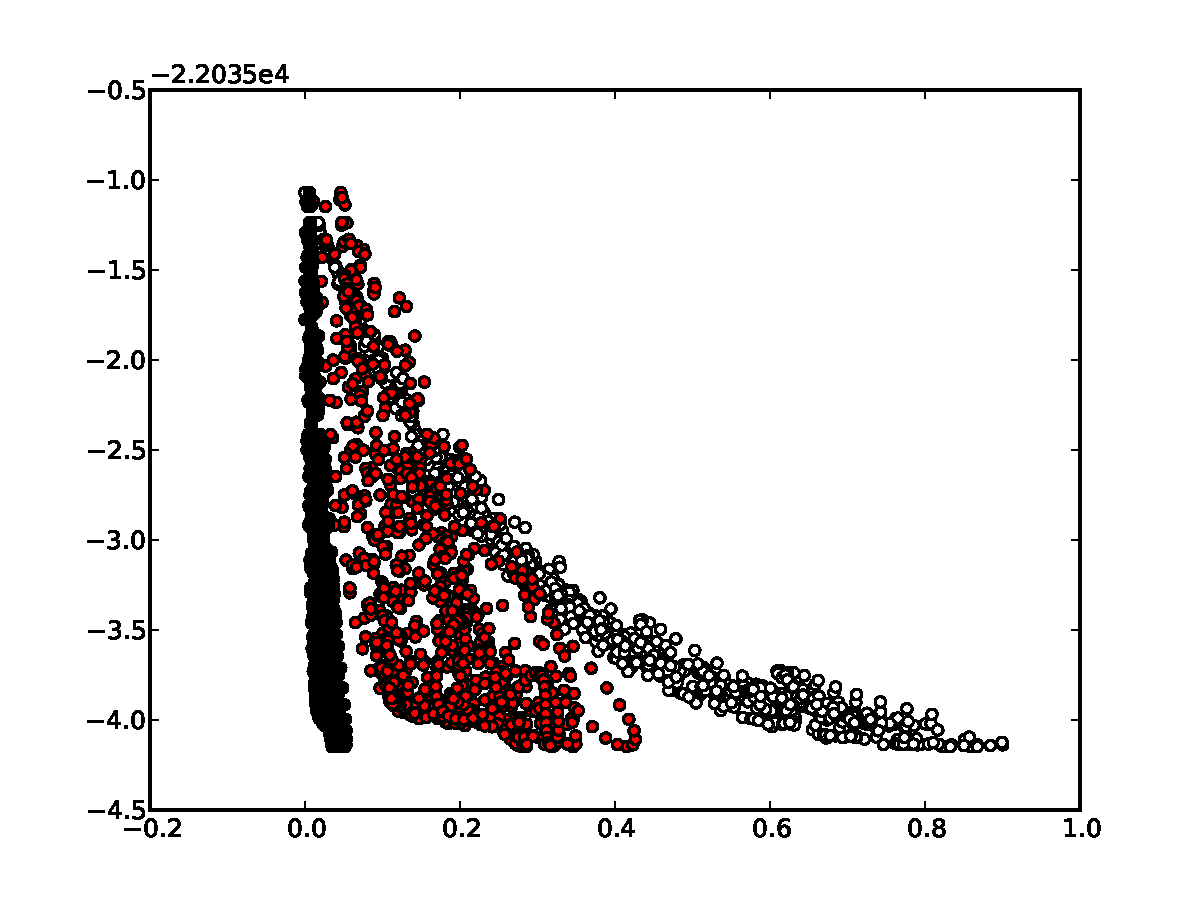
\includegraphics[width=0.35\linewidth]{h-mg-distances}
%    \label{fig:h-mg-distances}
%    }
%  \subfigure[\ce{Ca(BH4)2} energy profiles][\ce{Ca(BH4)2} energy profiles. The blue circles represent the $C_2$-type rotation and the red squares represent the $C_3$-type rotation.]{
%    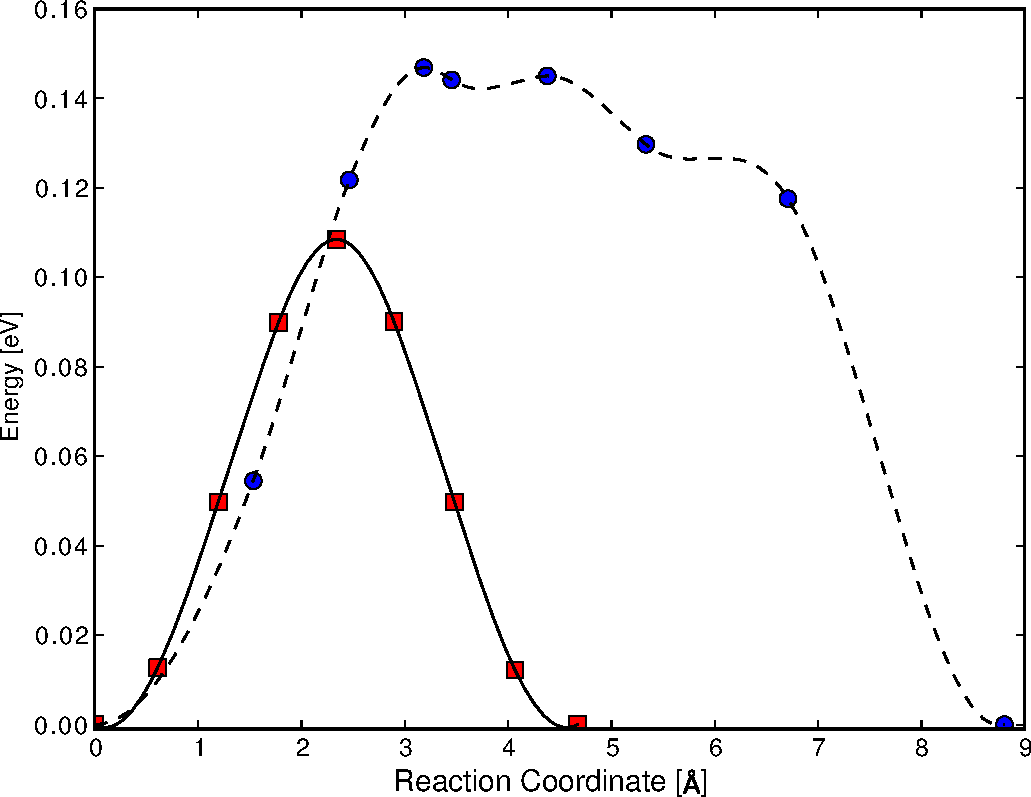
\includegraphics[width=0.45\linewidth]{ca-barriers}
%    \label{fig:ca-barriers}
%    }
    \parbox{0.85\linewidth}{
      \caption{qwer
      }
      \label{fig:h-mg-distances}
    }
\end{center}
\end{figure}


\figmiss{The different gengeral types of PESes.}

No such clear distinction could be made with regards to the $C_3$ axes.
However, due to symmetry all the $C_3$ axes for a given site yield a very similar PES. \tblue{(Should I show the four PESes for B04?)}

The rigid rotation plots are not able to give a full description of the events, neither their geometry nor their energetics.
Thus MEP calculations were performed with the lowest energy rigid rotation paths as starting guides.
The barriers from 

\figmiss{Barrier dependancy on distance}

It is unsurprising to find that there is a direct relationship between $L$ and the $C_2$ barrier height.
In fact, the relationship is linear, as can be seen in \fref{fig:mg-barriers}, with increased $L$ the barrier increases which is most likely due more \ce{H}-\ce{Mg} interaction.
On the other hand, no such direct relationship could be found for the $C_3$ axes.

\incomplete
